\chapter{Designing \& Engineering for Mobile}

\section{Aims}
\paragraph{} At the end of this topic you will be able to:

\begin{itemize}
\item Choose and follow a development methodology
\item Explain the mobile software development lifecycle
\item Perform Testing
\item Select the most appropriate development tools for your project
\end{itemize}


\paragraph{} We now focus on the practicalities of developing mobile apps in the wider context of software engineering and methodologies for creating effective and reliable software. Whilst in the last topic we considered the app in isolation with its own novel attributes in comparison to software on the server or desktop, instead, in this topic we consider how to engineer good apps and the methodologies we should follow if we are to build effective and reliable software. This is especially true if we consider thatin real-world development an app will rarely exist in isolation and will often be built by teams rather than individuals. An app will likely be part of a wider software system all of whose elements must work consistently together. Often an app will be developed which will work with data on the server, or services offered by 3rd parties, or will integrate closely with software on other platforms. Additionally, a team of developers working on a mobile app may have to work closely with developers building for other platforms or in different contexts. In order to make this process as smooth as possible, developers adopt software engineering methodologies and supporting tools to help them to work consistently and efficiently, to help them collaborate, and to ensure that their software artifacts are of high quality.

%SUPERHUB example.


\section{Methodologies}
\subsection{The Development Lifecycle}
\paragraph{} Developing mobile apps is simply software engineering in a specific application area. So what should our software engineering methods be?

\paragraph{} It is as if agile methods were made for mobile apps development. Short development cycles, building functionality and testing the app as you go along. The mantra is “test early, test often”. In agile, you can then stop when you have a product you can sell (or have run out of time and/ or money).

\paragraph{} Many software development projects start with a list of requirements generated from a customer/ client.  Often apps developers are drawing up their own requirements. Do a cost-benefit analysis on your project overall and of your requirements – prioritise them according to MOSCOW rules (those it must have, should have, could have and definitely won't have).

\begin{framed}
Planning to market your app? Don't forget any third-part requirements such as:
\begin{itemize}
\item Android License Agreement Requirements
\item Google Maps/ Third Party API Requirements
\item Android Market Requirements
\item Mobile Carrier/ Operator Requirements
\end{itemize}
\end{framed}

\paragraph{} A large, and underappreciated part of managing a software development project is managing risks. The biggest risk is your platform:
\begin{itemize}
\item handsets come and go at breakneck speed
\item handsets are customised for different markets \& regions
\item Android is at version 4.4 Kit-Kat– but for how long? each release is potentially significant to the success of your project
\item having access to the target handset – getting a pre-production handset might give you a competitive advantage
\end{itemize}

\paragraph{} Almost all of the most popular websites have migrated to phones – eg Facebook, BBC iPlayer – so simply expecting mobile users to browse to traditional websites is not seen as best practice for retaining your market share. Why's that?

\begin{itemize}
\item Small screen size – so need to customise
\item Limited/ uncomfortable data entry
\item Challenge of multitasking (eg Facebook is often running alongside MSN, YouTube on the desktop)
\item Representation of rich information (eg who's online, what's their strapline?)
\item Processor speed
\item Memory
\item Not always connected
\item Bandwidth
\item Expense of data roaming
\end{itemize}

\paragraph{} And from the users perspective?

\begin{itemize}
\item Interruptions likely – eg an SMS coming in
\item May be more public – more likely to be overlooked
\item May be more easily distracted
\item Need quick returns – some users download lots of apps but only use them infrequently
\end{itemize}

\subsubsection{Porting from a Desktop App} 
\paragraph{} 

\begin{itemize}
\item Avoid dialogs that pop up
\item Put interface elements under each other rather than side by side
\item To select a file – load them into a spinner
\item Test your app with one hand
\end{itemize}


\paragraph{} In summary, why are apps better than [web]sites for mobile? 
\begin{quote}
``Because the more impoverished the device, the more the design must be optimized for the platform's exact abilities, instead of bowing to a cross-platform common denominator.'' \footnote{\url{http://www.useit.com/alertbox/mobile-apps-initial-use.html}}
\end{quote}

\section{The Design Process}
\paragraph{} Jones \& Marsden (2006) define three activities involved in the design process:

\begin{itemize}
\item understanding users
\item developing prototype designs
\item evaluation – get feedback on your prototype and refine
\end{itemize}

\paragraph{} Overall, they state that interaction design should be “intensely participative and collaborative”. In most cases, to get the best results you can't go it alone – design reviews with peers and getting user feedback are useful in your app development.

\subsection{Understanding Users}
\paragraph{} To understand users you might want to conduct a field study. Ethnographers would study how people behave – taking into account collaboration, environment – observing how people behave in the situation in which the mobile app might be used. As an ethnographer you would be immersed in the environment and hopefully as invisible to the study group as possible.

\paragraph{} Do women and men behave differently? Course! Children and the elderly? The typical mobile user might not be an innovator and may not be a heavy desktop user. Your field study might observe different behaviours rather than making assumptions.

\paragraph{} Structured interviews/ direct questioning are more intrusive than ethnographic techniques, but are more direct and you can ask specific questions of your user group.

\paragraph{} How would these inform the design process? You could write up your observations \& interview results as scenarios (which are essentially use cases with more personality). This information would inform the prototyping stage as an indication of how the app could be used which in turn will inform the functionality required and the preferences in accessing/interacting with this functionality.

\subsection{Prototyping}

\paragraph{} The prototype is a basic working model of some part of an application which is either developed to get feedback into the requirements and/or design stage or which can be used as a step towards a final product. Developing a prototype is essential for mobile projects

\paragraph{} You can develop prototypes using mock up techniques (such mock-up.com, powerpoint templates, Visual Studio with Android plug-in, DroidDraw or Android App Inventor). 

\paragraph{} When developing your prototype, think about modelling the interaction with your final developed app. In particular (Jones \& Marsden,2006):
\begin{itemize}
\item direct manipulation – the iPod wheel is better than a scroll list
\item ecological use – would your context be useful eg location, other devices available to interact with eg over Bluetooth
\item design for maximum impact through minimum user effort
\item design for personalisation – people like to express their personality even though they are buying the same iPad as millions of others. Personalising makes them feel better towards their device/ app.
\item design for fun
\item design for one-handed use
\end{itemize}

\paragraph{} Add to that:

\begin{itemize}
\item design to be current OR functional (e.g. the Vuvuzela app for iPhone or the Bus Tracker – the former is use and throw away, the latter has currency through functionality)
\item use your mobile technology design guidelines\footnote{\url{http://developer.android.com/design/get-started/principles.html}} – e.g. Android offers a consistent framework for user interface components – well known ways of working with menus etc. Moving from one Android phone to another should be as easy as moving from one iPhone to another. There's no certification/ conformance rules yet but very strong guidelines on use of menus etc and icon style. They are protecting the brand.
\end{itemize}

\paragraph{} Guidelines are not just for display, guidelines are available for new gestures – the Android long press, iPhone’s pinch (now included in Android). Claiming to be intuitive, these new gestures are only intuitive if you first get shown them then all other devices use the same paradigm.
Some practical advice for apps developers:
\begin{itemize}
\item if possible, don't make users register first – hard lesson in ecommerce sites – let people put stuff in their basket before they fill out a form
\item try before you buy – or at least see before you buy
\item make it very simple – most app users are intermittent
\item include your icon design in this consideration – they might not use your app often – so make it easy for them to find when they do have the urge
\item design for performance – if you can get the work done by a server then farm it out, use efficient data structures, start fast, resume fast, use working progress tool
\item if possible, design for updates  - can extra features be plugged in without recompiling your app
\item design for interoperability  - can you work with other content providers
\item design in security – don't store or transmit non encrypted personal data
\item design for users on the go, being interrupted, having lots of apps
\end{itemize}

\subsection{Prototype Evaluation}
\paragraph{} Built your prototype? Now evaluate it – be ready to tear it up and start again – maybe you should let someone else evaluate? This is the hard bit – seeing your designs trashed. Develop a thick skin – and be a good listener. You don't always know best.

\paragraph{} Techniques include letting users loose on your prototype in a usability lab when they can be observed running through some sequence of operations. Then ask them to complete a questionnaire. You can also do some quantitative evaluation – how many keypresses are needed to run through the sequence, how long did it take etc

\paragraph{} You need enough functionality to make this prototype evaluation meaningful, however you don't want to complete your application only to find it's frustrating to use and won't sell.

\section{Development \& Testing}

\subsection{Development}
\paragraph{} Once you have established that your design is good – start developing. There’s nothing much that is particularly unique to Android app development:

\begin{itemize}
\item Pick the best IDE, i.e. Android Studio
\item Work long hours (but not silly hours)
\item FAQs and forums – if you haven’t got a google account, get one
\item Use code reviews to share good practice
\end{itemize}

\subsection{The Philosophy}

\paragraph{} The Android development philosophy includes insisting that you should keep resources external to your code where possible. Resources include strings and images. You can then look after them independently of your code. It also means that when a new device comes along with a screen shape you hadn’t anticipated you can make changes easily. Essentially: store everything in your resource directory (/res in Android Studio).


\begin{figure}[H]%[htb]
\centering
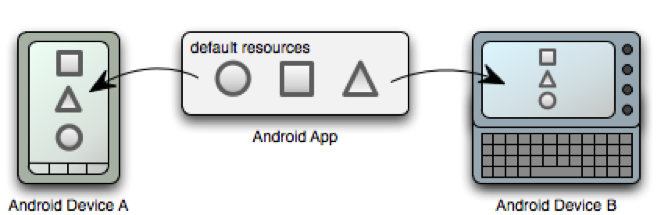
\includegraphics[width=\textwidth]{images/res_sharing}
\caption{Sharing Resources between devices}
\label{fig:res_sharing}
\end{figure}

\begin{figure}[H]%[htb]
\centering
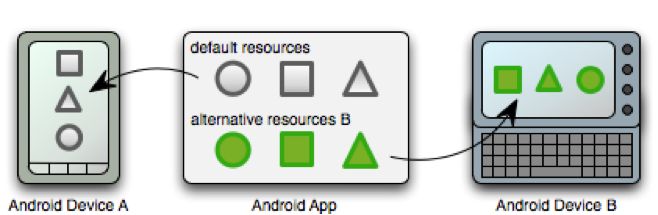
\includegraphics[width=\textwidth]{images/res_separate}
\caption{Using alternative resources for different devices}
\label{fig:res_separate}
\end{figure}


\begin{figure}[H]%[htb]
\centering
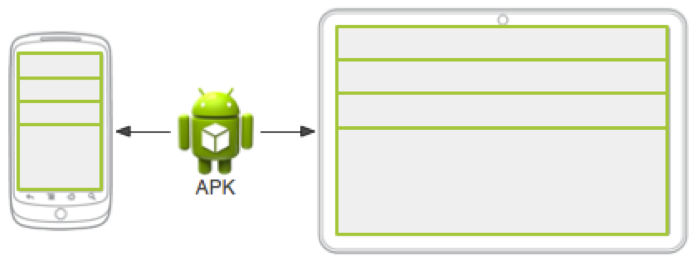
\includegraphics[width=\textwidth]{images/res-layout-default}
\caption{Resources resized - each using the default layout}
\label{fig:res-layout-defaultt}
\end{figure}

\begin{figure}[H]%[htb]
\centering
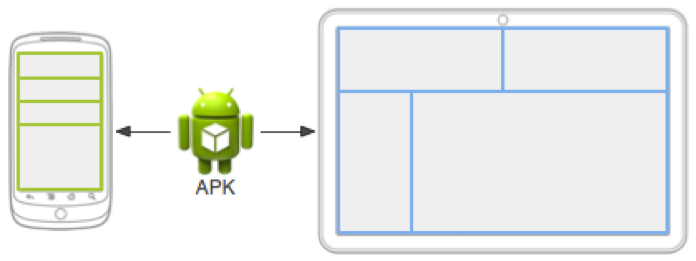
\includegraphics[width=\textwidth]{images/res-layout-alt}
\caption{Alternative layouts for tablets}
\label{fig:res-layout-alt}
\end{figure}

\subsection{Testing}
\paragraph{} As with agile methods, test early and often. To that we can add, for mobile apps, - try to test on your target kit as early as possible. Use a range of tools – such as JUnit and Android’s Monkey Exerciser. Monkey\footnote{\url{http://developer.android.com/guide/developing/tools/monkey.html}} is a command line tool which sends a random stream of events to your application to see how it deals with them. It can be used to stress test and can run on an emulator or a device. You can configure it to set up the number of events that should be created, to identify the packages you want to test, to establish event types and their frequencies and how it should react to an error. 

\begin{framed}
Why ``monkey''? From the infinite monkey theorem – if you have enough monkeys, at enough typewriters, eventually one of them will type the complete works of Shakespeare.
\end{framed}



\section{Tooling}
\paragraph{} There are many tools that can support you in creating robust and maintainable mobile apps. If we take Android as our example, there are the pre-requisites, basically Java and the Android SDK. You can develop for Android entirely at the command-line but there are also Integrated Development Environments (IDEs) which can help you. The two main IDEs are the Android SDK based on Eclipse which was historically been the default IDE for Android development and Android Studio which because the default IDE, according to the Android project, in December 2014. It is recommended that developers new to Android should work with Android Studio unless they are already higly experienced with Eclipse. Even then, it is difficult to say for how long the Eclipse Android plugins will continue to be supported.

However, you should always be aware that whilst these tools can help and support you, they are not a substitute for knowing the platform and the problem you are trying to solve, as well as possible. One advantage that IDEs to offer however is a way to explore the Android system by exploiting the visual editor, for drawing and prototyping layouts and exploring the view options without having to remember the XML that defines each option, and by exploiting the auto-complete feature which will suggest potential methods and objects from the Android libraries and your current project.

%\subsection{Integrated Development Environments}
%\subsubsection{Android Studio}
%\paragraph{} 

%\subsubsection{Eclipse with AndroidSDK plugin}
%\paragraph{}

\subsubsection{Build Control: Gradle \& Maven}
\paragraph{} Behind the more superficial UI differences between Studio and Eclipse, are some more substantial differences. One of the most important is the build system. Studio uses Gradle whereas Eclipse uses maven. An advantage of the new approach using Gradle is that various project parameters can be set in the Gradle build file which can then be used to complete your Android Manifest. This essentially means that you can have multiple Android apps built from the same codebase and build system, each targetting different API levels or working differently according to their target platform. This increases the flexibility of what was already a flexible system for developing apps to run across a wide range of platforms. Given that Android Studio uses Gradle, and Android Studio is the `tier one' development platform for Android, we should really get to grips with Gradle.

\subsection{Version Control}
\paragraph{} Version control is fundamental whether you are working individually or as part of a team. A good version control system, such as Git, will manage all of your resources and source code, enabling you to track changes between them, to track the history of each, and to maintain multiple versions of your app. Distributed version control, with sufficient tools for reconciling different and divergent versions, is essential when working with a team of developers, enabling each to work on their own part of the codebase and providing support to reconcile any `incompatible' difference between the versions. By incompatible versions we mean where developers have made alterations to the same piece of code and a decision has to be made about which to choose over the other, or whether refactoring to include both alterations is required. 

\subsubsection{Git}
\paragraph{} Unless you are already experienced with an alternative version control system, it is recommended that you use Git. There is a very good chance that during your career you will work in a software development team that uses this tool. Whilst Android Studio supports a range of version control tools, look under the ``VCS'' menu and you will see support for CVS, Subversion, Mercurial, and Git, Studio also supports GitHub which makes it straightforward to share your code, as open source for example, but also to create an offsite backup of your project.

\subsection{Best Practises}
\paragraph{} Due to the complicated Android hardware landscape there are many potential issues and pitfalls associated with developing app, particularly if you wish to reliable target a wide range of devices. The Android documentation provides a number of best practises\footnote{\url{https://developer.android.com/guide/practices/compatibility.html}} which it is worth becoming familiar with.

\paragraph{} For example,

\begin{itemize}
\item Use density-independent measurements in your layouts, so your specifications will scale along with the screen.
\item When putting together layouts, use relative widths and heights instead of absolute values.
\item Putting in several versions of the same image file, tailored to different screen densities, can also be a good idea.
\end{itemize}

\paragraph{} Because the Android eco-system is developing so rapidly it is worth trying to stay on top of the agreed best-practises and the differences between new versions of the platform. Whilst the platform APIs are quite rigid, to all intents and practises, if a feature is not supported by a particular API level then it is not available for that target, best practises are more malleable. It is always worth retaining a critical approach with respect to best practises and asking yourself, `does this still apply?', there may be a better way but it might be that nobody has realised it yet. Therefore best-practises can evolve and improve over time as the platform develops. This can be annoying, but means that the platform is still trying to innovate and be the best that it can be, even if sometime this means there must be major changes.

\section{Summary}
\paragraph{}

\paragraph{} In this topic we covered: 
\begin{itemize}
\item Designing your apps
\item Developing and testing your apps
\end{itemize}

\section{Directed Study}
\begin{itemize}
\item Read Chapters 4-6  of Mobile Interaction Design: Matt Jones \& Gary Marsden, Wiley, 2006
\item Read Chapters 18-19 of Android Wireless Application Development: Shane Condor \& Lauren Darcey, Addison-Wesley, 2010
\item Have a look at Microsoft’s guidelines  for their “metro style\footnote{\url{http://msdn.microsoft.com/library/windowsphone/develop/fa00461b-abe1-41d1-be87-0b0fe3d3389d(v=vs.105).aspx}}” for mobile apps and highlight any that wouldn’t be applicable to Android apps and visit the developers website http://developer.android.com for tips.
\item Check your understanding of the topic by answering the following:
\begin{enumerate}
\item Have you used design guidelines before (for example, in designing a website)? Can those be applied here?
\item What do interaction designers mean by “ethnography”?
\item If you are designing an app for older people, how would you contact a user group?
\item Why do you think SMS worked – beyond anyone's expectations?
\item Name 5 design rules built in to Android. Start by reading the Android design guidelines\footnote{\url{http://developer.android.com/guide/practices/ui_guidelines/index.html}}
\end{enumerate}
\item If you have time, build up an archive of your design ideas and inspiration from elsewhere – screen shots of killer apps, colour palettes, screen shots of your own work – critique your collection.
\end{itemize}


%\section{References \& Resources}
